 \documentclass[a4paper,fleqn]{cas-dc}

%%%Author definitions
\def\tsc#1{\csdef{#1}{\textsc{\lowercase{#1}}\xspace}}
\tsc{WGM}
\tsc{QE}
\tsc{EP}
\tsc{PMS}
\tsc{BEC}
\tsc{DE}
%%%

\usepackage[square,numbers,sort&compress,comma]{natbib}

\usepackage{amsmath}
\usepackage{amssymb}
\usepackage{diagbox}
\usepackage{caption}
\usepackage{graphicx}
\usepackage{latexsym}
\usepackage{times}
\usepackage[pagewise]{lineno}
\graphicspath{{figures/}}
\usepackage{color, colortbl}
\usepackage{chemformula}
\usepackage{xcolor}
\definecolor{Gray}{gray}{0.9}
\newcommand{\highlight}[1]{%
  \colorbox{Gray}{$\displaystyle#1$}}
\usepackage{color, colortbl}
\usepackage{chemformula}
\usepackage{xcolor}
\usepackage{adjustbox}
\usepackage{mathrsfs}
\usepackage{booktabs}
\usepackage{hyperref}
\usepackage{lipsum}

\emergencystretch = 0 pt
\pretolerance = 150
\tolerance = 250
\hbadness = 150
\hfuzz = 0 pt
\vfuzz = 0 pt

\usepackage{color}
\definecolor{color-strings}{rgb}{0,0,0.5}
\definecolor{color-keywords}{rgb}{0.6,0,0}
\definecolor{color-comments}{rgb}{0,0.5,0}
\definecolor{color-background}{rgb}{0.99,0.99,0.99}
\definecolor{color-numbers}{rgb}{0.7,0.7,0.7}
\definecolor{color-classes}{rgb}{0.2,0.3,0.4}

\usepackage{listings}
\lstdefinestyle{mystyle}{
	basicstyle=\ttm,
    backgroundcolor=\color{color-background},   
    commentstyle=\color{color-comments},
    keywordstyle=\color{color-keywords}\bfseries,
    numberstyle=\tiny\color{color-numbers},
    stringstyle=\color{color-strings},
    basicstyle=\linespread{0.8}\ttfamily\scriptsize,
    breakatwhitespace=false,         
    breaklines=true,                 
    captionpos=b,                    
    keepspaces=true,                 
    numbers=left,                    
    numbersep=5pt,                  
    showspaces=false,                
    showstringspaces=false,
    showtabs=false,                  
    tabsize=2,
    emph={Particle, FlowField, Image, Motion},
    emphstyle=\bfseries\color{color-classes},
}

\lstset{style=mystyle} 

\newcommand{ \kamila}[1]{\color{blue}{Kamila: #1} \color{black}}
\newcommand{ \todump}[1]{\color{olive}{#1} \color{black}}
\usepackage[normalem]{ulem}

\begin{document}

\shorttitle{\texttt{pykitPIV}: Rich and reproducible data generation for training machine learning algorithms in velocimetry}
\shortauthors{Zdyba\l{} et~al.}


\title [mode = title]{\texttt{pykitPIV}: Rich and reproducible data generation for training machine learning algorithms in velocimetry}

\author[EMPA]{Kamila Zdyba\l{}*}
\ead{kamila.zdybal@gmail.com}

\author[EMPA]{Claudio Mucignat}
\author[EMPA]{Stefan Kunz}
\author[EMPA]{Ivan Lunati}

\address[EMPA]{Laboratory for Computational Engineering, Swiss Federal Laboratories for Materials Science and Technology, Empa, Dübendorf, Switzerland}

\begin{abstract}
We describe \texttt{pykitPIV}, a Python library for generating synthetic images that mimic those obtained from particle image velocimetry (PIV) and background-oriented Schlieren (BOS) experimental techniques in fluid dynamics. The library integrates with machine learning (ML) algorithms, such as convolutional neural networks, variational approaches, active learning, or reinforcement learning. Our goal is to support the current trends in the velocimetry community for faster and more accurate real-time experimental inference, moving the field towards autonomous experimentation and building ML models from data. Our image generation exploits the kinematic relationship between two PIV/BOS snapshots, advecting particles from one time frame to the next with a second-order accurate numerical scheme. This results in paired image intensities, $(I_1, I_2)$, separated by $\Delta t$ in time. The goal of this library is to give the user, or the ML agent, flexibility in selecting various parameters that would normally be available in an experimental setting, such as seeding density, properties of the laser plane, camera exposure, particle loss, or experimental noise. We also provide an atlas of challenging synthetic velocity fields from analytic formulations. The effects of particle drift and diffusion in stationary isotropic turbulence can also be added atop the velocity fields using the simplified Langevin model. The richness of experimental conditions and reproducibility of image generation can help advance the growing development of ML applications in experimental fluid dynamics.
\end{abstract}

\begin{keywords}
particle image velocimetry; flow estimation; convolutional neural networks; machine learning; Python; PyTorch
\end{keywords}

\maketitle

\section{Motivation and significance\label{sec:introduction}}

The last decade has seen advances in training convolutional neural networks (CNNs) for optical flow estimation, \textit{i.e.}, predicting motion information from recorded image frames separated by a short time interval. To date, numerous network architectures have been developed that are highly specialized for this application. These include various implementations of FlowNets \citep{dosovitskiy2015flownet, ilg2017flownet, hui2018liteflownet}, the spatial pyramid network (SPyNet) \cite{ranjan2017optical}, the pyramid, warping, and cost-volume network (PWC-Net) \cite{sun2018pwc}, and, more recently, the recurrent all-pairs field transforms (RAFT) \cite{teed2020raft}. In addition, the introduction of iterative residual refinement (IRR) \cite{hur2019iterative} allowed for a significant reduction in the number of trainable parameters thanks to weight sharing at several levels of successively upscaled image resolution.

Experimental fluid dynamics can especially profit from those architectures. Specifically, particle image velocimetry (PIV) and background-oriented Schlieren (BOS) are experimental techniques used to visualize flow patterns with high precision. Their main goal is to predict flow targets, such as displacement fields, velocity components, or vorticity, either from paired snapshots of illuminated tracer particles injected into the flow (PIV) or from recorded deformations of the dotted background image. Recently, RAFT-PIV \cite{lagemann2021deep} and lightweight image-matching architecture (LIMA) \citep{manickathan2023lightweight} were proposed as versions of CNNs that are further optimized for inference from velocimetry experiments. Thanks to their targeted architecture and parameters, both RAFT-PIV and LIMA achieve high accuracy and per-pixel spatial resolution. The successes of RAFT-PIV and LIMA have been demonstrated on a number of classic experimental fluid dynamics settings such as flow behind a cylinder, boundary layer flow, or convective flow of a hot air plume \cite{mucignat2023lightweight}.

% CNNs are the first "layer" of various other ML algorithms that can move us towards autonomous experimentation
Currently, the main precedence that motivates the need for those networks is that they can be trained on GPUs within the matter of hours and then ported to laboratory hardware to make flow predictions in real-time, parallel to experimental measurements. In fact, our group already uses LIMA in real-time for 15Hz PIV, but further improvements to inference speed are needed for higher image acquisition frequencies. The advancements to these architectures are continually being made in the context of PIV \citep{shan2024lightweight, elrefaie2024site}. The appealing goal of the PIV community is that CNNs replace and outperform state-of-the-art PIV post-processing in the future. As a result, CNNs can become an image-processing workhorse behind many other machine learning (ML) algorithms such as variational approaches (VA), active learning (AL), or reinforcement learning (RL), allowing the experimental community to explore many new research avenues, such as autonomous experimentation and enhanced flow control.

To advance the development and performance of ML algorithms for complex experimental applications, a number of research questions will have to be addressed in the future:
\begin{enumerate}
\item How rich should the training dataset be for a given experimental setting?
\item Are there extreme image generation settings at which the current CNNs would fail?
\item Can we generate new training data samples to accomplish transfer learning, \textit{i.e.}, to make a trained ML model applicable in the next experimental setting?
\item Can we extend CNN's range of applicability within a single experimental setting with active learning?
\item As ML for PIV post-processing becomes widely used, how do we make sure that training-data generation is reproducible and can be easily shared between research groups?
\end{enumerate}

\begin{figure*}[t]
\centering
\vspace{-0.4 in}
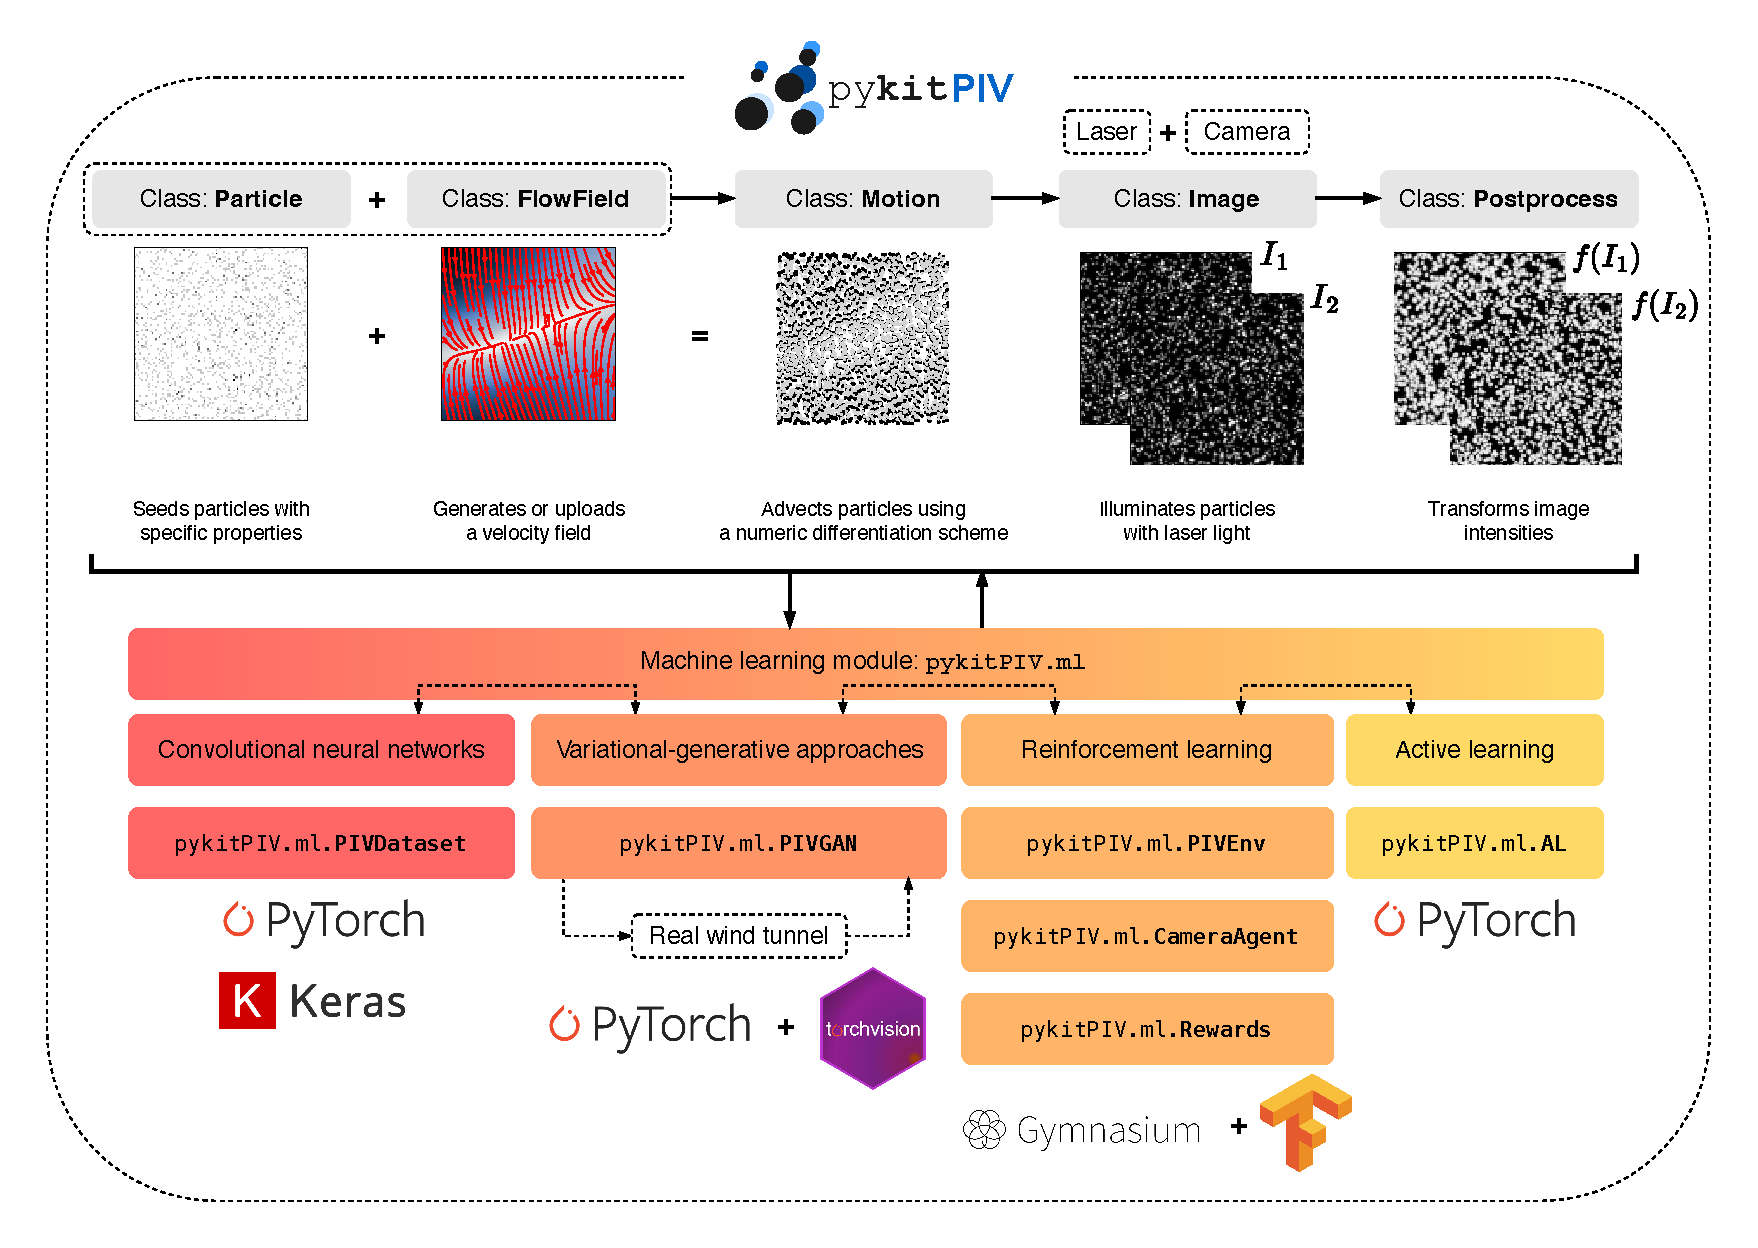
\includegraphics[width=\textwidth]{pykitPIV-modules.pdf}
\vspace{10 pt}
\caption{\footnotesize Order of using the five main \texttt{pykitPIV} classes. At each stage of synthetic image generation, the user has freedom in selecting various parameters that would normally be available in an experimental setting such as seeding density, properties of the laser plane, camera exposure, particle loss, or experimental noise.}
\label{fig:pykitPIV-overview}
\end{figure*}

To help researchers answer those questions, in this paper, we describe \texttt{pykitPIV} (\textbf{Py}thon \textbf{ki}nematic \textbf{t}raining for \textbf{PIV}), a Python library for synthetic PIV image generation that allows to create rich and challenging experimental scenarios. The library generates paired image intensities, $I_1$ and $I_2$, separated by $\Delta t$ in time, and the corresponding displacement fields, $d\mathbf{s} = [d \mathbf{x}, d\mathbf{y}]$ that have per-pixel resolution by construction. \texttt{pykitPIV} exploits the kinematic relationship between two consecutive PIV image frames \cite{manickathan2022kinematic}. Given any velocity field, tracer particles are advected from one time frame to the next using a second-order accurate numerical scheme. \texttt{pykitPIV} thus provides experiment-like images and the associated post-processing targets (\textit{e.g.}, $d\mathbf{s}$) which establish the ground truth for ML algorithms. This is in contrast to raw experimental data which lacks the ground truth. In fact, synthetic dataset are scarce and often do not exploit challenging flow scenarios. \texttt{pykitPIV} addresses this gap and allows for rich experimental conditions to be generated and presented to ML algorithms as batches of data.

To date, we have been able to identify four openly-available synthetic image generation (SIG) packages: one written in the ANSI C language coming from the EUROPIV project \cite{lecordier2004europiv}, two written in MATLAB \citep{ben2020openpiv, mendes2020piv}, and third package, implemented in both MATLAB and Python, with a limited scope in order to specifically track defocusing and tackle astigmatic PIV. These existing SIG implementations make integrating with Python interfaces more difficult. With the emerging ML applications, a package that readily ports to libraries such as PyTorch \cite{paszke2017automatic, paszke2019pytorch}, TensorFlow \cite{tensorflow2015}, or Keras \cite{chollet2015keras} is the ideal solution. Our library allows for easier porting with ML algorithms. This not only allows to generate training data for ML in a single Python workflow, but also allows the ML algorithm to interact with the image generation process. Specifically, the high flexibility in the types of created images can port very well with variational approaches (VA) or with reinforcement learning (RL) algorithms, where an agent may learn to augment the training dataset in real-time to account for changes in experimental settings. Within the tutorials provided with the software, we delineate interesting examples for each of these ML applications.

ML algorithms for PIV are often trained using synthetic images generated with open-source realistic flowfields, \textit{e.g.}, taken from the John Hopkins Turbulence Database (JHTD) \cite{perlman2007data}. While the JHTD database is openly available, the synthetic image generation is often performed by different groups using in-house codes. We have hopes that providing \texttt{pykitPIV} as an open-source Python library, researchers can easily share their image generation workflows, making the training of ML algorithms fully reproducible.

Notably, our library can integrate with the post-processing Python software developed in \cite{aguilar2022dpivsoft}.

%Finally, the powerful novelty of this package, as compared to previous MATLAB-based packages, is the introduction of new adjustable parameters that mimic various aspects of the experimental settings. 

%\cite{mucignat2024respiratory}

\section{Software description} \label{sec:software}

%For example, we provide the user with four types of experimental noise including shot noise. 
%We also provide a naive translation of images generated using classic optical cameras to event-based cameras.

%LIMA is also significantly leaner in terms of the number of trainable parameters than its predecessors used for general-purpose optical flow estimation. 

\subsection{Software architecture}

All functionalities of \texttt{pykitPIV} are organized in five classes: \texttt{Particle}, \texttt{FlowField}, \texttt{Motion}, \texttt{Image}, and \texttt{Postprocess}, each achieving its own role in generating synthetic image pairs and the corresponding flow targets. Fig.~\ref{fig:pykitPIV-overview} illustrates the hierarchy of using \texttt{pykitPIV} classes and briefly describes what can be achieved with each class. The user selects the number of image pairs to generate (batch size) and their dimensions (height and width). At each stage of image generation, the user can fix random seeds to assure that data generation is reproducible. Image properties are Monte-Carlo-generated and individual images within a training batch can span a range of conditions. Beyond the five main classes, we provide a dedicated ML module, \texttt{pykitPIV.ml}, which contains wrappers and integrations to various ML algorithms.



\subsection{Software functionalities}

The \texttt{Particle} class seeds the two-dimensional flow domain with tracer particles. The user can steer the range of particle diameters and their standard deviation, the seeding density, or the average distances between particles. The initial particle positions are those appearing on snapshots $I_1$.

The \texttt{FlowField} class allows to generate the velocity field to be applied on the two-dimensional domain. We implemented several methods to generate velocity fields, such as random smooth field, checkered field, Chebyshev polynomial field, or spherical harmonics field. Those are illustratively visualized in Fig.~\ref{fig:velocity-fields}a-d. This variety of velocity fields span cases with smooth and sharp velocity gradients and can help put machine learning algorithms to test. The user also has the option of uploading an external velocity field, \textit{e.g.}, coming from a numerical simulation of Navier-Stokes equations (\textit{cf.} Fig.~\ref{fig:velocity-fields}e), or coming from a synthetic turbulence generator (\textit{cf.} Fig.~\ref{fig:velocity-fields}f) \citep{saad2017scalable, richards2018fast}.

\begin{figure}[t]
\centering
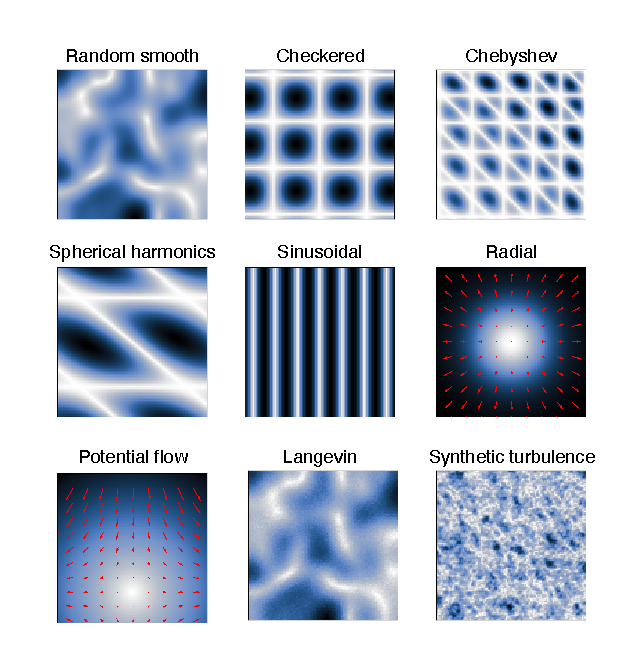
\includegraphics[width=9cm]{velocity-fields.pdf}
\caption{\textbf{a}-\textbf{e}: Types of two-dimensional velocity fields that can be generated with the \texttt{FlowField} class. \textbf{f}: The user also has the option to upload an external velocity field, \textit{e.g.}, coming from synthetic turbulence.}
\label{fig:velocity-fields}
\end{figure}

The \texttt{Motion} class applies the flow field to the particles. It uses a forward Euler or the Runge-Kutta 4th order numeric scheme to advect particles by a user-specified time separation, $\Delta t$. Velocity components in-between the grid points are interpolated with a regular grid interpolation. The main output of this class are particle positions that will appear on snapshots $I_2$, each paired with a respective snapshot $I_1$.

\begin{figure}[t]
\centering
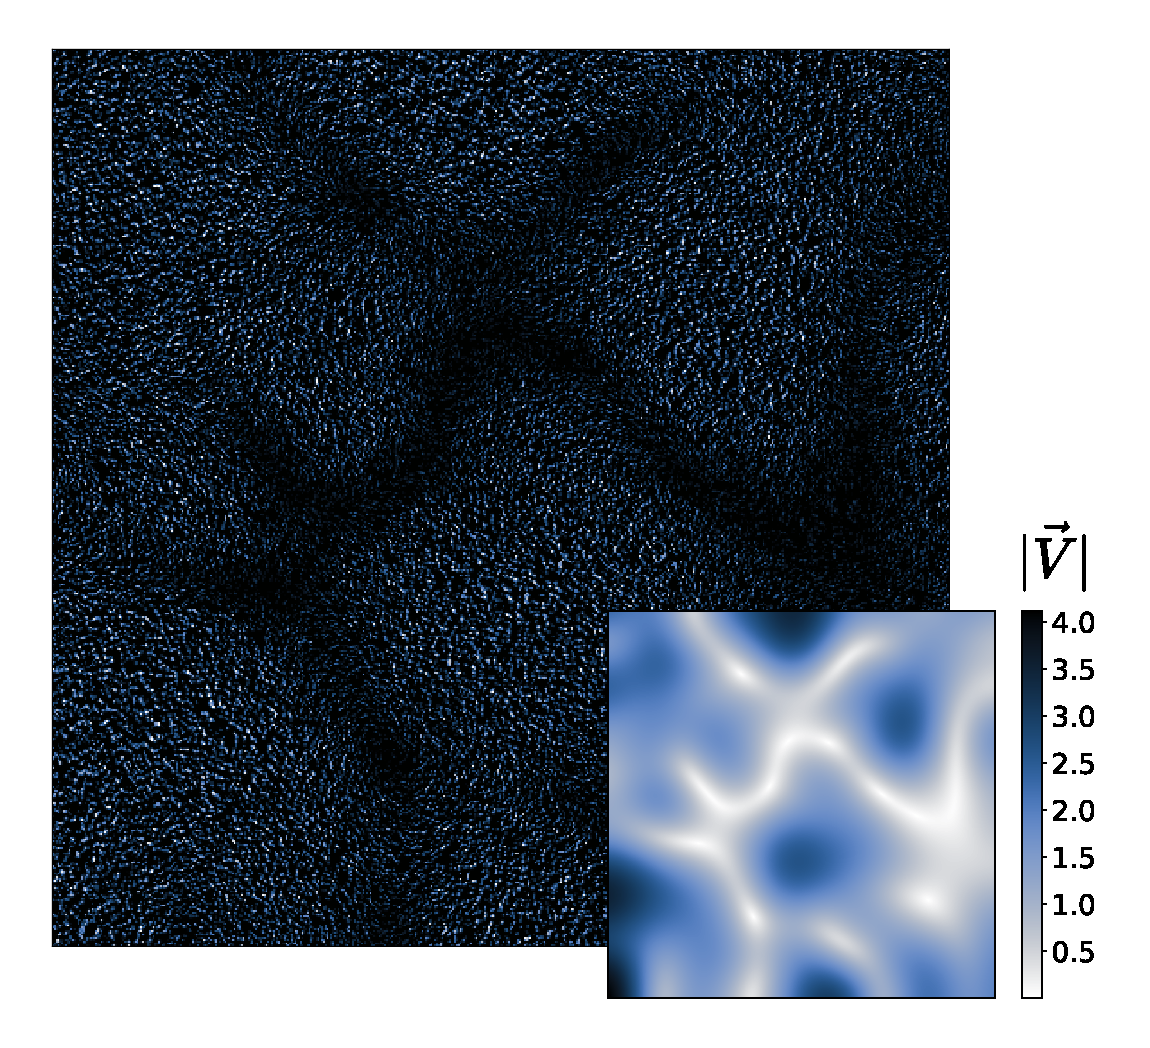
\includegraphics[width=8cm]{motion-image.pdf}
\caption{Example visualization of particle motion resulting from superimposing $I_1$ and $-I_2$ on one image and given the velocity magnitude, $|\vec{V}|$.}
\label{fig:particle-motion}
\end{figure}

The \texttt{Image} class generates image intensities. It adds the reflected laser light to the generated PIV image pairs. The core functionality is to add a Gaussian intensity to each particle \citep{olsen2000out, rabault2017performing}. The user has a lot of flexibility in setting up the laser plane and camera properties. The user can also steer the amount of particles lost between frame $I_1$ and $I_2$ due to out-of-plane movement.

The PIV image pair tensor has shape $(N, 2, H, W)$, where $N$ is the batch size, $H$ is image height and $W$ is image width. The second dimension can be thought of as the number of channels and those correspond to $I_1$ and $I_2$, respectively. This is compatible with tensor shape accepted by convolutional layers implemented in PyTorch (\texttt{torch.nn.Conv2d}). Note that the whole batch of $N$ images can be generated all at once or can be optimized for memory and generated in batches. The \texttt{Image} class contains convenient functions for saving images to \texttt{.h5} files and for plotting or animating image pairs. \texttt{pykitPIV} uses sequential colormaps by Crameri et al. \cite{crameri2020misuse}.

The \texttt{Postprocess} class contains functions that apply transformations to generated images. It can be especially useful for data augmentation, where the training dataset is extended with images with various levels of noise or illumination levels.

\section{Illustrative examples} \label{sec:examples}

Below, we present the most straightforward workflow for generating a batch of $N=100$ PIV image pairs and their associated targets and we save the resulting tensors for later use in PyTorch. Each image is 256px $\times$ 256px. We create a 10px boundary buffer during image generation to allow for new particles to enter the image area and hence to prevent spurious disappearance of particles near image boundaries.

We import \texttt{pykitPIV}'s classes and specify the global parameters:
\lstset{language=Python}
\begin{lstlisting}
from pykitPIV import Particle, FlowField, Motion, Image

n_images = 100
image_size = (256, 256)
size_buffer = 10
random_seed = 100
\end{lstlisting}
We instantiate an object of the \texttt{Particle} class:
\lstset{language=Python}
\begin{lstlisting}
particles = Particle(n_images,
                     size=image_size,
                     size_buffer=size_buffer,
                     diameters=(4,4.1),
                     distances=(1,2),
                     densities=(0.05,0.1),
                     diameter_std=0.2,
                     seeding_mode='random',
                     random_seed=random_seed)
\end{lstlisting}
We instantiate an object of the FlowField class and we generate random smooth velocity fields for each of the $N=100$ image pairs:
\lstset{language=Python}
\begin{lstlisting}
flowfield = FlowField(n_images,
                      size=image_size,
                      size_buffer=size_buffer,
                      random_seed=random_seed)

flowfield.generate_random_velocity_field(
				gaussian_filters=(10,11),
				n_gaussian_filter_iter=10,
				displacement=(2,10))
\end{lstlisting}
We instantiate an object of the \texttt{Motion} class and we run a forward Euler numerical scheme to advect the particles:
\lstset{language=Python}
\begin{lstlisting}
motion = Motion(particles, 
                flowfield, 
                time_separation=0.1)
                
motion.forward_euler(n_steps=10)
\end{lstlisting}
Finally, we instantiate an object of the \texttt{Image} class, add particles, flow field, and motion objects and add reflected light with the specific laser plane properties:
\lstset{language=Python}
\begin{lstlisting}
image = Image(random_seed=random_seed)

# Add particles to images:
image.add_particles(particles)

# Add flow field to images:
image.add_flowfield(flowfield)

# Add motion to images:        
image.add_motion(motion)

# Add reflected light to images:
image.add_reflected_light(exposures=(0.7,0.8),
                          maximum_intensity=2**16-1,
                          laser_beam_thickness=1,
                          laser_over_exposure=1,
                          laser_beam_shape=0.95,
                          alpha=1/10)
\end{lstlisting}
Once all images are created, we can remove buffers from the images, convert image pairs and the flow targets to tensors, and save tensors to \texttt{.h5} files for future use:
\lstset{language=Python}
\begin{lstlisting}
# Remove image buffers:
image.remove_buffers()

# Prepare image tensors:
image_pairs = image.image_pairs_to_tensor()
targets = image.targets_to_tensor()

# Save images to .h5:
image.save_to_h5({'I': image_pairs, 
							'targets': targets}, 
							filename='PIV-dataset.h5')
\end{lstlisting}

\section{Impact} \label{sec:results}

The kinematic training methodology \cite{manickathan2022kinematic}, which is the core concept behind generating PIV image pairs with \texttt{pykitPIV}, has been used to train CNNs in optical flow estimation \cite{manickathan2022kinematic, manickathan2023lightweight, mucignat2023lightweight}. The approach proved successful, which suggests that for small enough $\Delta t$, learning the kinematic relationship between two consecutive PIV snapshots, as opposed to knowing the full dynamic relationship, is sufficient to train CNNs.




\kamila{It would be great if we could extend image generation to synthetic event-based camera datasets. This would make the software truly novel.}

\kamila{Perhaps a nice novelty would be to allow the user to add solid boundaries into the image?}


\subsection{Porting with convolutional neural networks}

\kamila{Here we can describe what can be achieved in terms of training a CNN.}

\subsection{Porting with reinforcement learning}

\kamila{Here we can describe what can be achieved in terms of training an RL agent, e.g. in the context of autonomous experimentation. Maybe the agent will learn to augment the dataset in real time to account for changing experimental settings.}


\section{Conclusions}


We plan a continued development of this library.

Future application can also include the use variational approaches to inform training data collection, or train a RL agent to construct necessary support data in new environments.

\section*{Declaration of competing interest}

The authors declare that they have no known competing financial interests or personal relationships that could have appeared to influence the work reported in this paper.

\section*{Author contributions}



\section*{Acknowledgments}



\bibliographystyle{pci}
\bibliography{bibliography}

\end{document}